\lecture{10}{1. April 2025}{Motorer og gasturbiner}

\section{Motorer og gasturbiner}
Dette kapitel vil omhandle de gas-baserede kredsprocesser med intern forbrænding i modsætning til de faseskift-baserede kredsprocesser med ekstern forbrænding præsenteret i \autoref{afs:kraftværk}: \nameref{afs:kraftværk}. Dette kan grundlæggende opdeles i de tre principper:
\begin{itemize}
  \item Benzinmotoren (Otto-princippet)
  \item Dieselmotoren (Diesel-princippet)
  \item Gasturbinen (Brayton-princippet)
\end{itemize}

\subsection{Beregningsforudsætninger}
En række forudsætninger vil nu blive præsenteret for at lette arbejdsgangen (undgå mange iterationer). De overordnede principper kan dog i teorien godt overføres til et mere virkelighedsnært scenarie, såfremt man husker at tage højde for de øvrige variable.

\subsubsection{Arbejdsmediet i anlægget}
Dette kapitel vil se nærmere på tre typer anlæg, som kan karakteriseres på følgende principper:
\begin{enumerate}
  \item De er \underline{arbejdsproducerende}, hvilket vil sige, at formålet med at bygge anlæggene er at producere akseleffekt, som efterfølgende kan udnyttes til eksempelvis at drive en generator eller anden arbejdskonsumerende maskineri
  \item Energiinputtet stammer fra en \underline{intern forbrænding}, hvilket vil sige, at et brændstof forbrændes direkte i mediet i anlægget, hvoraf der kan bære både luft og røggas tilstede i maskinen
  \item Mediet eller medierne i anlægget er overalt på \underline{gasform}
\end{enumerate}
For at lette beregningerne på anlæggene kan opstilles følgende forudsætninger:
\begin{enumerate}
  \item Arbejdsmediet overalt i anlægget kan antages at være tør atmosfærisk luft, som cirkulerer i kredsprocessen
  \item Alle delprocesser er reversible
  \item Den interne forbrændingsproces erstattes af en ekstern forbrænding, og varmen fra forbrændingen overføres til arbejdsmediet i anlægget ved varmeveksling
  \item Udstødningsprocessen erstattes af en varmeafgivelsesproces, og varmen afgives fra arbejdsmediet i anlægget til omgivelserne ved varmeveksling
  \item De specifikke varmekapaciteter $c_p$ og $c_v$ antages uafhængige af temperaturen og derved anses for konstante. Isentropeksponenten $\kappa$ vil således være konstant
\end{enumerate}

\subsubsection{Stempelmaskiner}
Benzinmotoren (Otto-princippet) og Dieselmotoren (Diesel-princippet) er i de fleste tilfælde cylinder-stempel maskiner eller forkortet til stempelmaskiner (Wankelmotorer er eksemeplvis ikke), hvor der er behov for at definere en række geometridata.

\begin{figure} [ht]
  \centering
  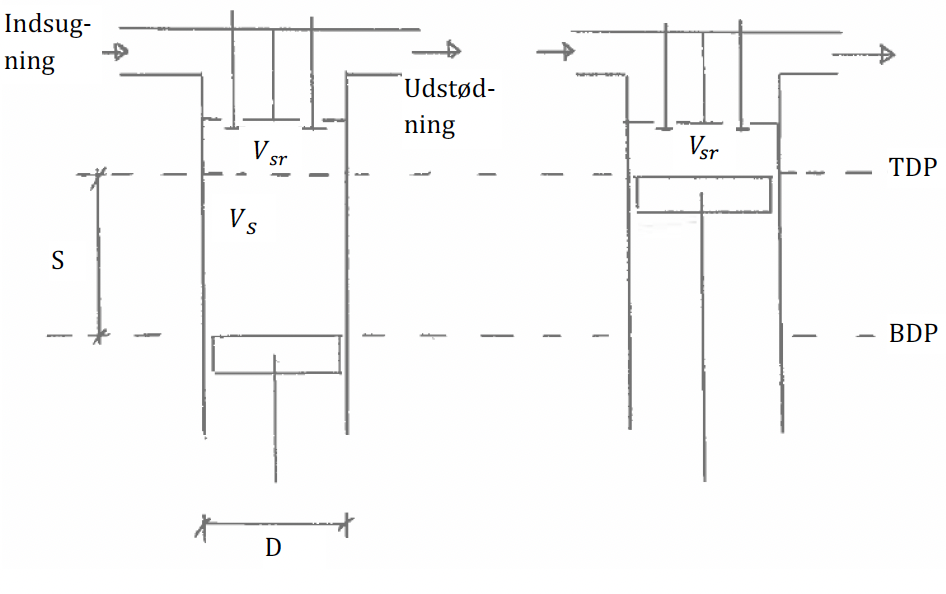
\includegraphics[width=0.5\linewidth]{./figures/f10_1.png}
  \caption{Snit af et cylinder-stempel system}
  \label{fig:f10_1}
\end{figure}

På \textbf{\autoref{fig:f10_1}} er vist et snitbillede af et cylinder-stempel system. Stemplet i systemet bevæger sig mellem \textit{bunddødpunktet} (BDP) og \textit{topdødpunktet} (TDP). I en virkelig motor er indsugnings- og udstødningsventilens opgave hhv. at tilføre forbrændingsluft fra omgivelserne til cylinderen og bortlede forbrændingsgasser eller røggasser fra cylinderen til omgivelserne.

Når stemplet er i TDP forefindes et volumen i cylinderen som benævnes \textit{det skadelige rum} $V_{s r}$ eller det døde rum. Det skadelige rum har dette lidt negative navn, idet det ikke bidrager positivt til kredsprocessen. Størrelsen af det skadelige rum defineres af konstruktøren af motoren.

Volumenet mellem BDP og TDP kaldes for slagvolumenet $V_s$. Slagvolumenet kan bestemmes idet $D$ er den indvendige diameter af cylinderen og $S$ er slaglængden, som:
\[ 
V_s = \frac{\pi}{4} \cdot D^2 \cdot S
.\]
Kompressionsforholdet $r$ som man skal bemærke sig, er et volumenforhold og ikke et trykforhold defineres som:
\[ 
r = \frac{\text{Største volumen i cylinderen}}{\text{Mindste volumen i cylinderen}} = \frac{V_s + V_{sr}}{V_{s r}}
.\]

Akseleffekten fra motoren $\dot{W}_a$ bestemmes som:
\begin{align*}
  \dot{W}_a &= \eta_{\mathrm{mek}} \cdot N_c \cdot W_{v, \mathrm{kreds}} \cdot \frac{\unit{rpm}}{60} \cdot \left( \frac{2}{N_{\mathrm{takt}}} \right) \qquad \text{(reversible kredsprocesser)} \\
  \dot{W}_a &= \eta_{\mathrm{mek}} \cdot N_c \cdot W_{g, \mathrm{kreds}} \cdot \frac{\unit{rpm}}{60} \cdot \left( \frac{2}{N_{\mathrm{takt}}} \right) \qquad \text{(generelt)}
.\end{align*}
Hvor $\eta_{\mathrm{mek}}$ er den mekaniske virkningsgrad for motoren (typisk \num{0,75}--\num{0,90}), $N_c$ er antallet af cylindere, $W_{v, \mathrm{kreds}}$ er det for gassen på stemplet udøvede kredsarbejde for en reversibel proces uden dissipationsarbejde. $W_{g, \mathrm{kreds}}$ er dittoen men for reelle processer med dissipationsarbejde. $\unit{rpm}$ er omdrejningstallet og $N_{\mathrm{takt}}$ er antallet af takter i kredsprocessen (2- eller 4-takts motor).

Den mekaniske virkningsgrad repræsenterer tabene mellem det for gassen på stemplet udøvede netto kredsarbejde og akselarbejdet på krumtapakslen $W_a$. Antages delprocesserne for gassen i cylinderen, som er et lukket system, for refversible kan det samlede arbejde for kredsprocessen $W_{g, \mathrm{kreds}}$ forenkles til volumenændringsarbejdet for kredsprocessen $W_{v, \mathrm{kreds}}$.

Faktoren $\frac{2}{N_{\mathrm{takt}}}$ er et ``formeltrick'' som korrigerer for hvor mange omdrejninger krumtakakslen tager for en kredsproces. En 2-takt motor tager en omdrejning på krumtapakslen for hver kredsproces, mens en 4-takts motor tager 2.

Massen af den indespærrede luftmængde i cylinderen kan findes vha. idealgasligningen, hvis sammenhængende værdier af $p, T, V$ kendes. I mange tilfælde kender man dette efter indsugning, hvor det kan antages at tilstanden i cylinderen er $p = p_0, T = T_0, V = V_{s r} + V_s$. Derefter kan idealgasligningen bruges til at finde massen af luften som:
\[ 
m = \frac{p \cdot V}{R_i \cdot T}
.\]

\subsection{Otto-motoren}

\subsubsection{Otto-motorens virkemåde}
Benzinmotoren arbejder efter det såkaldte \textit{Otto-princip} eller \textit{gnisttændingsprincippet}. En blanding af forstøvet benzin og luft suges via indsugningsventilen ind i cylinderen, og komprimeres før det antændes af et tændrør. Derfor omtaler man Otto-motoren som en \textit{gnisttændingsmotor}. Betragtes et cylinder-stempel system i en 4-taks benzinmotor er det grundlæggende princip at:
\begin{itemize}
  \item Halv rotation af krumtapakslen: Stemplet bevæges opad fra BDP til TDP og der sker en kompression af luft og benzinblandingen i cylinderen
  \item Yderligere en halv rotation: Forbrænding sker efter gnisttænding og trykket stiger i cylinderen. Stemplet bevæges nedad fra TDP til BDP og der sker en ekspansion af røggassen i cylinderen
  \item Yderligere en halv rotation: Stemplet bevæger sig opad fra BDP til TDP og idet udstødningsventilen åbner, vil røggassen blive trykket ud til omgivelserne. Udstødningsventilen lukkes igen
  \item Yderligere en halv rotation: Stemplet bevæger sig nedad fra TDP til BDP og idet indsugningsventilen åbnes, vil frisk luft- og benzinblanding blive suget ind i motoren fra karburatoren, hvor blandingen af luft og benzin sker i det rigtige forhold. Indsugningsventilen lukkes igen
\end{itemize}

For en 2-takts benzinmotor er princippet:
\begin{itemize}
  \item omtrent \ang{120} rotation: Stemplet bevæger sig nedad fra TDP mod BDP efter en forbrænding og der sker en ekspansion af røggassen i cylinderen
  \item Yderligere \ang{90} rotation: Stemplet vender bevægelsesretning ved BDP, og idet udstødningsventilen åbnes vil røggassen blive trykket ud til omgivelserne. Lukning af udstødningsventilen påbegyndes, så indsugningsventilen kan åbnes. Herfra vil luft og forstøvet benzin blive suget ind i motoren fra krumtaphuset. Denne indstrømningsluft hjælper også med at tømme cylinderen for røggas, hvorved en vis opblanding af luft- og benzinblandingen og den producerede røggas vil forekomme. Derefter lukkes indsugningen igen
  \item Yderligere \ang{90} rotation: Stemplet bevæger sig opad mod TDP og der sker en kompression af luft og benzinblandingen i cylinderen
  \item yderligere ca. \ang{60} rotation: Stemplet bevæger sig fortsat opad til TDP og der sker en forbrænding efter gnisttænding og trykket stiger i cylinderen
\end{itemize}

\begin{figure} [ht]
  \centering
  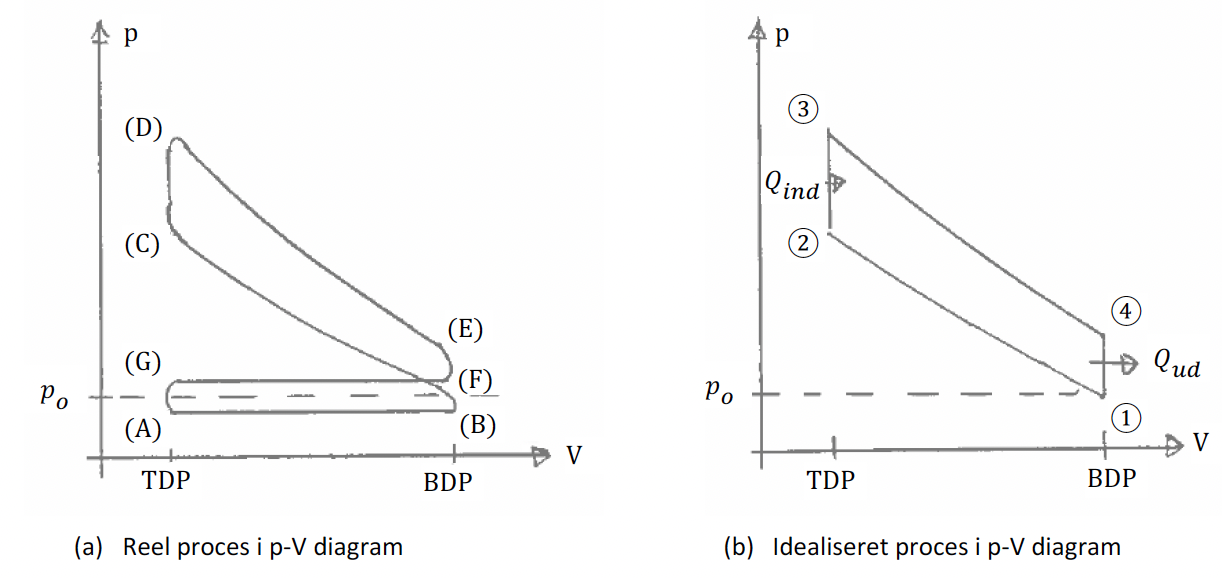
\includegraphics[width=0.5\linewidth]{./figures/f10_2.png}
  \caption{$p$-$V$ diagrammer for benzinmotorer efter 4-taktprincippet}
  \label{fig:f10_2}
\end{figure}

På \textbf{\autoref{fig:f10_2}} er vist et $p$-$V$ diagram både for en virkelig benzinmotor og efter en idealiseret benzinmotor. Begge er efter 4-taktprincippet. På $V$-aksen er TDP og BDP angivet, mens omgivelsestrykket $p_0$ er angivet på $p$-aksen. Her kan et par karakteristika for den virkelige proces observeres:
\begin{itemize}
  \item Pkt. A til B: Den vandrette kurve under omgivelsestrykket $p_0$, hvor procesvejen går fra TDP mod BDP, repræsenterer indsugningen. Trykket er lavere end omgivelsestrykket, da der på en virkelig motor vil være tryktab over karburator og indsugningsventil
  \item Pkt B til C/D: Procesvejen går fra BDP mod TDP, og repræsenterer komprimering, hvor trykket stiger og specielt ved afslutningen af komprimeringen, hvor der sker forbrænding fra C til D
  \item Pkt. D til E/F: Procesvejen går fra TDP mod BDP, og repræsenterer ekspansion, hvor trykket falder og specielt ved afslutningen af ekspansionen, hvor der sker udstødning fra E til F
  \item Pkt. F til G: Den vandrette kurve over omgivelsestrykket $p_0$, hvor procesvejen går fra BDP mod TDP, repræsenterer udstøgning. Trykket er højere end omgivelsestrykket, da der på en virkelig motor vil være tryktab over udstødningsventil og det øvrige udstødningssystem. 
\end{itemize}

Arealet $BCDEF$ i \textbf{\autoref{fig:f10_2}} repræsenterer et positivt bidrag til arbejdet udført af kredsprocessen, mens arealet $ABFG$ repræsenterer et negativt bidrag til arbejdet udført af kredsprocessen, idet dette areal er en konsekvens ved indsugning og udstødning. 

På \textbf{\autoref{fig:f10_2}} er der som tidligere nævnt også præsenteret et $p$-$V$ diagram for en idealiseret 4-takts proces efter Otto-princippwt. Arealet $ABFG$ er udeladt, idet det antages, at der ikke er tryktab i motoren. Den idealiserede kredsproces består af de fire delprocesser:
\begin{itemize}
  \item Pkt. 1 til 2: Isentropisk kompression
  \item Pkt. 2 til 3: Isokorisk varmetilførsel
  \item Pkt. 3 til 4: Isentropisk ekspansion
  \item Pkt. 4 til 1: Isokorisk varmeafgivelse
\end{itemize}
Det antages videre at tætningen mellem cylinder og stempel er perfekt således, at der ikke sker lækage af gas internt i motoren. At alle delprocesserne er reversible, hvilket indebærer, at der ikke er friktion og derved tryktab internt i motoren. At kompressionen og ekspansionen sker som en quasi-stationær tilstandsændring, dvs. tilpas langsomt, så der kan nå at ske perfekt trukudligning i cylinderen. Slutteligt antages at alle komponenter er adiabatiske -- på nær dem for hvilke, der skal ske varmeveksling. Man kan generelt finde volumenarbejdet i kredsprocessen som:
\[ 
W_{v, \mathrm{kreds}} = - \left( Q_{23} + Q_{41} \right) = m \cdot c_{v, 23} \cdot \left( T_2 - T_3 \right) + m \cdot c_{v, 41} \cdot \left( T_4 - T_1 \right) 
.\]
Hvis man antager en konstant specifik varmekapacitet kan det ovenstående reduceres til:
\[ 
W_{v, \mathrm{kreds}} = m \cdot c_{v} \cdot \left( T_2 - T_3 + T_4 - T_1 \right) 
.\]

\subsubsection{Idealiseret beregningsprocedure -- volumenændringsarbejdet, akselarbejde}
Nettoarbejdet af kredsprocesen kan findes som summen af arbejdet ved hver delproces. For et lukket reversibelt system må der således være tale om volumenændringsarbejdet og følgende formel kan opstilles:
\[ 
W_{\mathrm{net}} = W_{v, \mathrm{kreds}} = \sum W_{v}
.\]
Volumenændringsarbejdet for hver delproces er:
\begin{align*}
  W_{v, 12} &= \frac{m \cdot R_i \cdot \left( T_2 - T_1 \right) }{\kappa - 1}\\
  W_{v, 34} &= \frac{m \cdot R_i \cdot \left( T_4 - T_3 \right) }{\kappa - 1} \\
  W_{v, 23} &= W_{v, 41} = 0
.\end{align*}
Med ovenstående procedure bliver $W_{v, 12}$ positivt og v.v. for $W_{v, 34}$. Da $W_{v, 34}$ er større end $W_{v, 12}$ vil $W_{v, \mathrm{kreds}}$ per konvention være negativ.

\subsubsection{Idealiseret beregningsprocedure, virkningsgrad}
Den termiske virkningsgrad for benzinmotoren kan defineres som:
\[ 
\eta_{th, \mathrm{Otto}} = \frac{\text{Ønsket output}}{\text{Nødvendigt input}} = \frac{\left| W_{\mathrm{net}} \right|}{Q_{23}} = 1 - \left( \frac{V_2}{V_1} \right)^{\kappa - 1} = 1 - \frac{1}{r^{\kappa - 1}}
.\]
Hvor $r$ er kompressionsforholdet.

Benzinmotorer bygges normalt med et kompressionsforhold i intervallet $[8;11]$. Dette skyldes at virkningsgraden forøges for større kompressionsforhold. Man kan ikke normalt have kompressionsforhold over omtrent 11, da blandingen så vil blive så varm at den kan selvantænde, hvilket kaldes \textit{tændingsbankning}.


\subsection{Diesel motoren}

\subsubsection{Dieselmotorens virkemåde}
Dieselmotorer arbejder efter \textit{Diesel-princippet} eller \textit{kompressionstændingsprincippet}. Det er alene luft, som suges ind i cylinderen via indsugningsventilen, og dieselolien sprøjtes ind i cylinderen via en dyse umiddelbart før der er behov for en forbrænding. Antænding af den forstøvede dieselolie i luften sker udelukkende som følge af den forhøjede temperatur ved komprimering af luften. Disse kan også arbejde efter både 2-taktprincippet og 4-taktprincippet. 

\begin{figure} [ht]
  \centering
  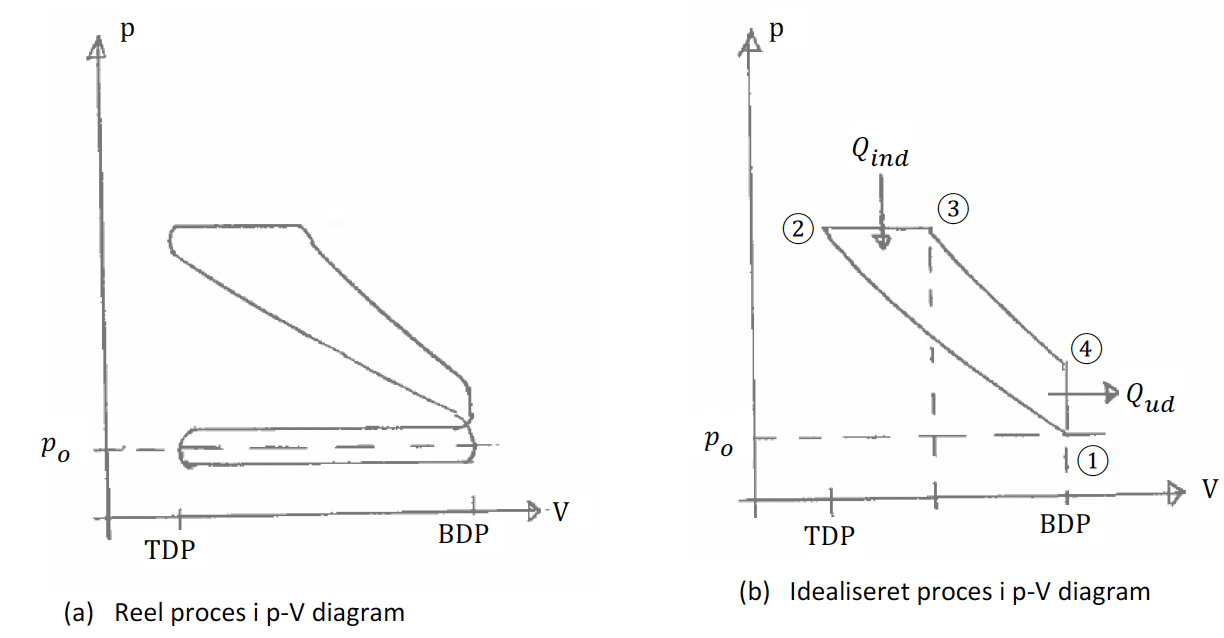
\includegraphics[width=0.5\linewidth]{./figures/f10_3.png}
  \caption{$p$-$V$ diagrammer for dieselmotorer efter 4-taktprincippet}
  \label{fig:f10_3}
\end{figure}

På \textbf{\autoref{fig:f10_3}}. Her er BDP og TDP igen indtegnet på $V$-aksen og omgivelsestrykket $p_0$ er anført på $p$-aksen. Det ses hurtigt at dieselmotoren adskiller sig fra benzinmotoren ved at forbrændingen sker således, at st stemplets nedadgående bevægelse resulterer i, at trykket holdes tilnærmelsesvis konstant, og en del af kredsprocessen kan beskrives som en isobar proces.

\subsubsection{Idealiseret beregningsprocedure -- varmebalancemetoden, akselarbejde}
Den idealiserede kredsproces på \textbf{\autoref{fig:f10_3}} består af følgende 4 delprocesser
\begin{itemize}
  \item Pkt. 1 til 2: Isentropisk kompression
  \item Pkt. 2 til 3: Isobarisk varmetilførsel
  \item Pkt. 3 til 4: Isentropisk ekspansion
  \item Pkt 4 til 1: Isokorisk varmeafgivelse
\end{itemize}

For pkt. 3 benævnes volumenet for \textit{cut-off volumenet} $V_c$. Med afsæt i dette har man, for dieselmotorer, defineret det såkaldte \textit{cut-off forhold} som:
\[ 
r_c = \frac{V_c}{C_{s r}}
.\]
Volumenarbejdet kan her findes som:
\[ 
W_{v, \mathrm{kreds}} = -\left( Q_{23} + Q_{41} \right) = m \cdot c_{p,23} \cdot \left( T_2 - T_3 \right) + m \cdot c_{v, 41} \cdot \left( T_4 - T_1 \right) 
.\]
Eller for en specifik varmekapacitet som:
\[ 
W_{v, \mathrm{kreds}} = m \cdot c_{p} \cdot \left( T_2 - T_3 \right) + m \cdot c_v \cdot \left( T_4 - T_1 \right) 
.\]

\subsubsection{Idealiseret beregningsprocedure -- volumenændringsarbejdsmetoden, akselarbejde}
Også for dieselmotorer er det samlede volumenændringsarbejde $W_{\mathrm{net}}$ blot summen af arbejdet for hver delproces som:
\[ 
W_{\mathrm{net}} = W_{v, \mathrm{kreds}} = \sum W_{v}
.\]
Og for hver delproces har vi:
\begin{align*}
  W_{v, 12} &= \frac{m\cdot R_i \cdot \left( T_2 - T_1 \right) }{\kappa - 1} \\
  W_{v, 23} &= p_2 \cdot \left( V_2 - V_3 \right)  \\
  W_{v, 34} &= \frac{m \cdot R_i \cdot \left( T_4 - T_3 \right) }{\kappa - 1} \\
  W_{v, 41} &= 0
.\end{align*}
Her vil $W_{v, \mathrm{kreds}}$ også blive negativ per konvention som var tilfældet for Ottoprocessen. 

\subsubsection{Idealiseret beregningsprocedure, virkningsgrad}
Den termiske virkningsgrad for dieselmotoren er defineret som:
\[ 
\eta_{t, \mathrm{Diesel}} = \frac{\text{Ønsket output}}{\text{Nødvendigt input}} = \frac{\left| W_{\mathrm{net}} \right|}{Q_{23}}
.\]
Hvilket kan vises at være givet ved:
\[ 
\eta_{th, \mathrm{Diesel}} = 1 - \frac{1}{r^{\kappa - 1}} \cdot \left( \frac{r_c^{\kappa} - 1}{\kappa \left( r_c - 1 \right) } \right)
.\]
Det kan i øvrigt vises, at for cut-off ratio gående mod 0 $r_c \to 0$ vil den termiske virkningsgrad for dieselmotorer gå mod den for en tilsvarende benzinmotor. Idet tændingsbankning ikke er et problem for dieselmotorer sættes deres kompressionsforhold dog typisk i intervallet $[13;24]$.


\subsection{Gasturbinen}

\subsubsection{Gasturbinens opbygning og virkemåde}
En gasturbine adskiller sig opbygningsmæssigt væsentligt fra en benzin- og dieselmotor. Gasturbinen består i stedet af en kompressor og turbine koblet på samme aksel. Mellem disse to er er et brændkammer, hvor brændslet forbrændes. Dette er vist på \textbf{\autoref{fig:f10_4}}.

\begin{figure} [ht]
  \centering
  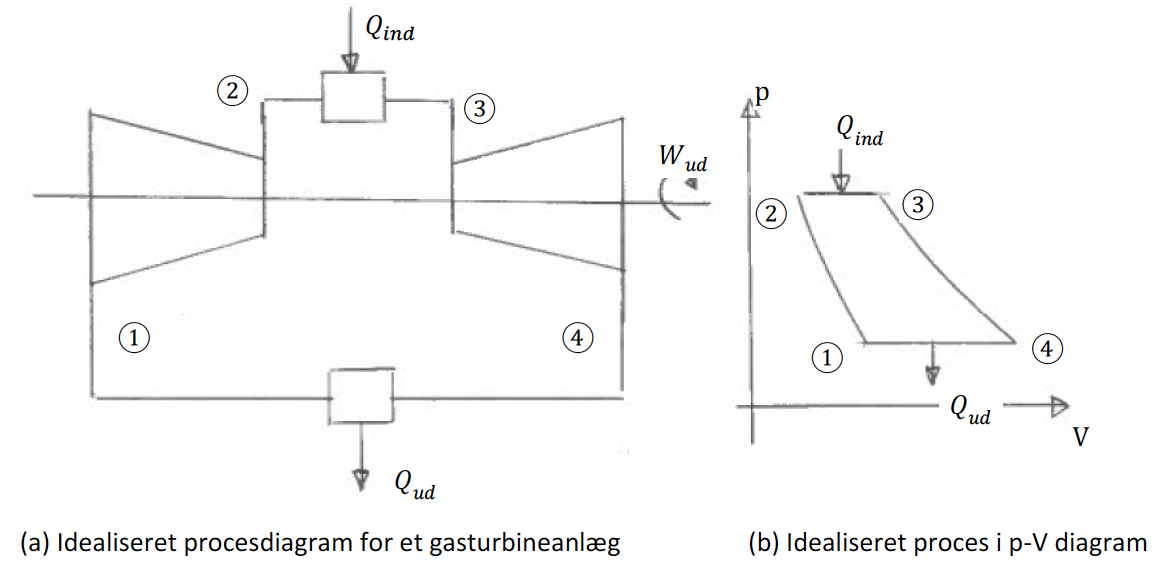
\includegraphics[width=0.5\linewidth]{./figures/f10_4.png}
  \caption{Procesdiagram for en gasturbine}
  \label{fig:f10_4}
\end{figure}

Det er naturligvis ikke alle brændsler, som kan benyttes i et gasturbineanlæg, og det må kræves, at andelen af partikler eller aske i brændslet er lille. Typiske brændsler i et gasturbineanlæg er naturgas, propan eller lette fossile olier. Kul har med et askeindhold på omtrent 3-20\% for højt et askeindhold til at være nyttigt i en gasturbine.

På \textbf{\autoref{fig:f10_4}} er vist et idealiseret og teoretisk procesdiagram for et gasturbineanlæg, som vil lette beregningerne på anlægget. Det antages at gasturbineanlgget kører mellem to trykniveauer og at tør atmodsfærisk luft cirkulerer i en lukket kreds. Ved det høje tryk er forbrændingen erstattet af en isobarisk varmetilførselsproces. Ved det lave tryk er udstødningen erstattet af en isobarisk varmeafgivelsesproces. Denne samlede proces benævnes til tider \textit{Brayton-princippet}.

\subsubsection{Idealiseret beregningsprocedure ‐ varmebalancemetoden, akselarbejde}
Kredsprocessen kan deles op i følgende 4 delprocesser:
\begin{itemize}
  \item Pkt. 1 til 2: Isentropisk kompression
  \item Pkt. 2 til 3: Isobarisk varmetilførsel
  \item Pkt. 3 til 4: Isentropisk ekspansion
  \item Pkt. 4 til 1: Isobarisk varmeafgivelse
\end{itemize}
For gasturbiner har man i øvrigt defineret det såkaldte \textit{trykforhold} $r_p$ givet ved:
\[ 
r_p = \frac{p_2}{p_1}
.\]
Her fås det tekniske arbejde til:
\[ 
W_{t, \mathrm{kreds}} = - \left( Q_{23} + Q_{41} \right) = m \cdot c_{p,23} \cdot \left( T_2 - T_3 \right) + m \cdot c_{p,41} \cdot \left( T_4 - T_1 \right)
.\]
Hvis der antages en konstant specifik varmekapacitet reduceres dette til:
\[ 
W_{t, \mathrm{kreds}} = m \cdot c_p \cdot \left( \left( T_2 - T_3 \right) + \left( T_4 - T_1 \right)  \right) 
.\]

\subsubsection{Idealiseret beregningsprocedure ‐ volumenændringsarbejdsmetoden, akselarbejde}
Også her er kredsprocessens samlede nettoarbejde summen af de indågende delprocesser som:
\[ 
W_{\mathrm{net}} = W_{t, \mathrm{kreds}} = W_{v, \mathrm{kreds}} = \sum W_v
.\]
Og arbejdet for hver af de 4 delprocesser er:
\begin{align*}
  W_{v, 12} &= \frac{m \cdot R_i \cdot \left( T_2 - T_1 \right) }{\kappa - 1} \\
  W_{v, 23} &= p_2 \cdot \left( V_3 - V_2 \right)  \\
  W_{v, 34} &= \frac{m \cdot R_i \cdot \left( T_4 - T_3 \right) }{\kappa - 1} \\
  W_{v, 41} &= p_4 \cdot \left( V_1 - V_4 \right) 
.\end{align*}
Igen her er resultatet per konvention negativt.

\subsubsection{Idealiseret beregningsprocedure, virkningsgrad}
Den termiske virkningsgrad for en gasturbine er defineret som:
\[ 
\eta_{th, \mathrm{Brayton}} = \frac{\text{Ønsket output}}{\text{Nødvendigt input}} = \frac{\left| W_{\mathrm{net}} \right|}{Q_{23}}
.\]
Hvilket kan vises at svare til:
\[ 
\eta_{th, \mathrm{Brayton}} = 1 - \frac{1}{r_p^{\frac{\kappa - 1}{\kappa}}}
.\]
Dette er den maksimalt opnåelige virkningsgrad under de givne forhold. I England og USA har man tradition for at udtrykke ``godheden'' af specielt en gasturbine ved at danne forholdet mellem forbrugt brændstofsenergi og produceret akselenergi -- dette benævnes \textit{heat rete} $\mathrm{HR} \unit{\frac{kJ}{kWh}}$. Denne er defineret som:
\[ 
\mathrm{HR} = \frac{\dot{Q}_{\text{brændstof}} \unit{kW} \cdot \unit{\frac{J}{W\cdot s}}}{\left| \dot{W}_a \right| \unit{kW} \cdot \unit{\frac{h}{3600s}}} = \frac{\dot{Q}_{\text{brændstof}}}{\left| \dot{W}_{net} \right|}
.\]
Man bør være opmærksom på om producenten har brugt akselarbejdet $\dot{W}_a$ eller kredsarbejdet $W_{\mathrm{net}}$ til at beregne deres heat rate, idet forskellen på disse er tab i maskinen. 
